%%%%%%%%%%%%%%%%%%%%%%%%%%%%%%%%%%%%%%%%
% Structured General Purpose Assignment
% LaTeX Template
%
% This template has been downloaded from:
% http://www.latextemplates.com
%
% Original author:
% Ted Pavlic (http://www.tedpavlic.com)
%
% Note:
% The \lipsum[#] commands throughout this template generate dummy text
% to fill the template out. These commands should all be removed when 
% writing assignment content.
%
%%%%%%%%%%%%%%%%%%%%%%%%%%%%%%%%%%%%%%%%%

%----------------------------------------------------------------------------------------
%       PACKAGES AND OTHER DOCUMENT CONFIGURATIONS
%----------------------------------------------------------------------------------------

\documentclass{article}

\usepackage{fancyhdr} % Required for custom headers
\usepackage{lastpage} % Required to determine the last page for the footer
\usepackage{extramarks} % Required for headers and footers
\usepackage{graphicx} % Required to insert images
\usepackage{lipsum} % Used for inserting dummy 'Lorem ipsum' text into the template
\usepackage{subcaption}


\usepackage{amsmath}

% Margins
\topmargin=-0.45in
\evensidemargin=0in
\oddsidemargin=0in
\textwidth=6.5in
\textheight=9.0in
\headsep=0.25in 

\linespread{1.1} % Line spacing

% Set up the header and footer
\pagestyle{fancy}
\lhead{\hmwkAuthorName} % Top left header
\chead{\hmwkClass\ : \hmwkTitle} % Top center header
\rhead{\firstxmark} % Top right header
\lfoot{\lastxmark} % Bottom left footer
\cfoot{} % Bottom center footer
\rfoot{Page\ \thepage\ of\ \pageref{LastPage}} % Bottom right footer
\renewcommand\headrulewidth{0.4pt} % Size of the header rule
\renewcommand\footrulewidth{0.4pt} % Size of the footer rule

\setlength\parindent{0pt} % Removes all indentation from paragraphs

%----------------------------------------------------------------------------------------
%       DOCUMENT STRUCTURE COMMANDS
%       Skip this unless you know what you're doing
%----------------------------------------------------------------------------------------

% Header and footer for when a page split occurs within a problem environment
\newcommand{\enterProblemHeader}[1]{
\nobreak\extramarks{#1}{#1 continued on next page\ldots}\nobreak
\nobreak\extramarks{#1 (continued)}{#1 continued on next page\ldots}\nobreak
}

% Header and footer for when a page split occurs between problem environments
\newcommand{\exitProblemHeader}[1]{
\nobreak\extramarks{#1 (continued)}{#1 continued on next page\ldots}\nobreak
\nobreak\extramarks{#1}{}\nobreak
}

\setcounter{secnumdepth}{0} % Removes default section numbers
\newcounter{homeworkProblemCounter} % Creates a counter to keep track of the number of problems

\newcommand{\homeworkProblemName}{}
\newenvironment{homeworkProblem}[1][Problem \arabic{homeworkProblemCounter}]{ % Makes a new environment called homeworkProblem which takes 1 argument (custom name) but the default is "Problem #"
\stepcounter{homeworkProblemCounter} % Increase counter for number of problems
\renewcommand{\homeworkProblemName}{#1} % Assign \homeworkProblemName the name of the problem
\section{\homeworkProblemName} % Make a section in the document with the custom problem count
\enterProblemHeader{\homeworkProblemName} % Header and footer within the environment
}{
\exitProblemHeader{\homeworkProblemName} % Header and footer after the environment
}

\newcommand{\problemAnswer}[1]{ % Defines the problem answer command with the content as the only argument
\noindent\framebox[\columnwidth][c]{\begin{minipage}{0.98\columnwidth}#1\end{minipage}} % Makes the box around the problem answer and puts the content inside
}

\newcommand{\homeworkSectionName}{}
\newenvironment{homeworkSection}[1]{ % New environment for sections within homework problems, takes 1 argument - the name of the section
\renewcommand{\homeworkSectionName}{#1} % Assign \homeworkSectionName to the name of the section from the environment argument
\subsection{\homeworkSectionName} % Make a subsection with the custom name of the subsection
\enterProblemHeader{\homeworkProblemName\ [\homeworkSectionName]} % Header and footer within the environment
}{
\enterProblemHeader{\homeworkProblemName} % Header and footer after the environment
}
   
%----------------------------------------------------------------------------------------
%       NAME AND CLASS SECTION
%----------------------------------------------------------------------------------------

\newcommand{\hmwkTitle}{Assignment\ \#3 } % Assignment title
\newcommand{\hmwkDueDate}{Saturday,\ October\ 17,\ 2015(One late day used)} % Due date
\newcommand{\hmwkClass}{CSCI-567} % Course/class
\newcommand{\hmwkClassTime}{} % Class/lecture time
\newcommand{\hmwkAuthorName}{Saket Choudhary} % Your name
\newcommand{\hmwkAuthorID}{2170058637} % Teacher/lecturer
%----------------------------------------------------------------------------------------
%       TITLE PAGE
%----------------------------------------------------------------------------------------

\title{
\vspace{2in}
\textmd{\textbf{\hmwkClass:\ \hmwkTitle}}\\
\normalsize\vspace{0.1in}\small{Due\ on\ \hmwkDueDate}\\
\vspace{0.1in}\large{\textit{\hmwkClassTime}}
\vspace{3in}
}

\author{\textbf{\hmwkAuthorName} \\
        \textbf{\hmwkAuthorID}
        }
\date{} % Insert date here if you want it to appear below your name

%----------------------------------------------------------------------------------------

\begin{document}

\maketitle

%----------------------------------------------------------------------------------------
%       TABLE OF CONTENTS
%----------------------------------------------------------------------------------------

%\setcounter{tocdepth}{1} % Uncomment this line if you don't want subsections listed in the ToC

\newpage
\tableofcontents
\newpage


%----------------------------------------------------------------------------------------
%       PROBLEM 2
%----------------------------------------------------------------------------------------





\begin{homeworkProblem}[Problem 1] % Custom section title
\begin{homeworkSection}{\homeworkProblemName: ~(a)}

\problemAnswer{
	Let $\sigma(a) = \frac{1}{1+e^{-a}}$ and 
	
	$$ P(Y=1|X=x) = \sigma(b+w^Tx)\\
	\newline
	P(Y=0|X=x) = 1-\sigma(b+w^Tx)$$
	
	Observe that $Y=1$ when $b+w^Tx \geq 0$ and $Y=0$ when $b+w^Tx < 0$
	
	Thus,
	 
	\begin{align*}
	P(Y=y|X=x) &= \sigma(b+w^T)^y (1-\sigma(b+w^Tx))^({1-y})\\
	\log(P(Y=y|X=x)) &= y\log(\sigma(b+w^Tx))^y +  ({1-y}) \log(1-\sigma(b+w^Tx))\\
	&= y \log(\frac{\sigma(b+w^T)}{1-\sigma(b+w^Tx)}) + \log(1-\sigma(b+w^Tx))\\
	&= y(b+w^Tx) + \log(\frac{e^{-(b+w^Tx)}}{1+e^{-(b+w^Tx)}})\\
	&= y(b+w^Tx) + \log(\frac{1}{1+e^{(b+w^Tx)}})\\
	&= y(b+w^Tx) - \log(1+e^{(b+w^Tx)})\tag{[1.1]}
	\end{align*}
	
	\begin{align*}
		\mathcal{L}(\boldmath{w}) &= -\log(\prod_{i=1}^nP(Y=y_i|X=x_i))\\
		&= -\sum_{i=1}^n \log(P(Y=y_i|X=x_i))\\
		&= -\sum_{i=1}^n\big( \boldmath{y_i}(b+w^T\boldmath{x_i}) - \log(1+e^{(b+w^T\boldmath{x_i})})\big)\\
%		&= \sum_{i=1}^n\big( \boldmath{-y_i}(b+w^T\boldmath{x_i}) + \log(1+e^{(b+w^T\boldmath{x_i})})\big)\\
		%&= -\sum_{i=1}^n\big( \log(e^{(\boldmath{y_i}(b+w^T\boldmath{x_i}))}) - \log(1+e^{(b+w^T\boldmath{x_i})})\big)\\
		%&= -\sum_{i=1}^n\big( \log(e^{(\boldmath{y_i}(b+w^T\boldmath{x_i}))}) - \log(1+e^{-y_(b+w^T\boldmath{x_i})})\big)\\	
	\end{align*}
	
	
	Consider $\mathcal{L}(w) = -y(b+w^Tx) + \log(1+e^{(b+w^Tx_i)})$
	
	
	\begin{align*}
	\frac{\partial \mathcal{L}(w)}{\partial w} &= -(xy^T) + \frac{e^{(b+w^Tx)}x}{1+e^{(b+w^Tx)}}\\
	\frac{\partial^2 \mathcal{L}(w)}{\partial w^2}&= 0 +  \frac{\partial }{\partial w}\big(x-\frac{x}{1+e^{(b+w^Tx)}}\big)\\
	\frac{\partial^2 \mathcal{L}(w)}{\partial w^2}&= \frac{x(e^{(b+w^Tx)})x^T}{(1+e^{(b+w^Tx)})^2} \geq 0\ \forall\ x \in \mathbf{R}\\
	\frac{\partial^2 \mathcal{L}(w)}{\partial w^2}&= x^T \sigma(b+w^Tx)(1-\sigma(b+w^Tx))x \geq 0  \tag{1.2}\\
	\end{align*}
	
	From (1.2) $\frac{\partial^2 \mathcal{L}(w)}{\partial w^2} \geq 0$ and hence, from the definition of convex functions, $\mathcal{L}(w)$ is indeed a convex function.
	}
\end{homeworkSection}
\begin{homeworkSection}{\homeworkProblemName: ~(b)}

\problemAnswer{
	
	
	When the data is perfectly linearly separable, (assume first $n/2$ of the $n$ training points belong to class 0 and the remaining to class $1$), thus our regression model should assign the first $n/2$ points to class 1 with cent percent certainty or with probability 1 and the remaining $n/2$ to class 0 with probability 1.
	For this to happen, $P(Y=1|X=X_1) = 1$ and $P(Y=0|X=X_0)=1$ where $X_1$ is the set of points belonging to class $1$ and $X_0$ is the set of points belonging to class 0.
	
	Clearly this scenario is possible when $||w|| \longrightarrow \infty$
}
\end{homeworkSection}
\begin{homeworkSection}{\homeworkProblemName: ~(c)}
	\problemAnswer{

	A simple example with two points would be $(0,0)$, $(1,1)$. Intuitively the step function's step branches (the horizontals of a sigmoid function) will be located at infinity. Also the line separating the points (0,0) and (1,1) can be anywhere in between 0 and 1, thus there will be multiple solutions.
}
\end{homeworkSection}

\begin{homeworkSection}{\homeworkProblemName: ~(d)}
	\problemAnswer{
		\begin{align*}
		\mathcal{L}(w) &= \sum_{j=1}^n\big( \boldmath{-y_j}(b+w^T\boldmath{x_j}) + \log(1+e^{(b+w^T\boldmath{x_j})})\big) + \lambda ||w||_2^2\\
		\frac{\partial \mathcal{(L)}(w)}{\partial w_i} &=  \sum_{j=1}^n\big( \boldmath{-y_j}(\boldmath{x_{ji}}) + \frac{x_{ji}e^{(b+w^T\boldmath{x_j}) x_{ij}}}{1+e^{(b+w^T\boldmath{x_j})}}\big) + 2\lambda w_i = 0\\
		\frac{\partial^2 \mathcal{(L)}(w)}{\partial w_i^2} &=  \sum_{j=1}^n\big(  \frac{x_{ji}^2e^{(b+w^T\boldmath{x_j}) x_{ij}}}{(1+e^{(b+w^T\boldmath{x_j})})^2}\big) + 2\lambda > 0
		\end{align*}
		where the last inequality holds since $\lambda > 0$ 
		Consider $f(w_i) = \sum_{j=1}^n\big( \boldmath{-y_j}(\boldmath{x_{ji}}) + \frac{x_{ji}e^{(b+w^T\boldmath{x_j}) x_{ij}}}{1+e^{(b+w^T\boldmath{x_j})}}\big) + 2\lambda w_i = 0$
		
		And $u,v$ are the two solutions of $f(w_i)=0$, i.e. $f(u) = f(v) = 0$ (Without loss of generality, assume $u < v$)
		
		By Rolle's theorem, If $f(u)=f(v)=0$ then there exists a point in $[u,v]$ say $c$ such that $f'(c)=0$ for $c \in [u,v]$
		
		But, $f'(w_i) = \sum_{j=1}^n\big(  \frac{x_{ji}^2e^{(b+w^T\boldmath{x_j}) x_{ij}}}{(1+e^{(b+w^T\boldmath{x_j})})^2}\big) + 2\lambda > 0$
		and hence there exists no such $c$.
		
		and hence the function is convex, thus the solution to the partial differential $\frac{\partial \mathcal{(L)}(w)}{\partial w_i}$ is unique.
	}
\end{homeworkSection}
\end{homeworkProblem}

\begin{homeworkProblem}[Problem 2]
	\begin{homeworkSection}{\homeworkProblemName: ~(a)}
	\problemAnswer{
		Consider $||w||_0= \#{i: w_i \neq 0}$ for a 1D case.
		Where, $x_1=(0)$ and $x_2 = (\epsilon)$ where $0 < \epsilon << 1$
		
		$f(\boldmath{w}) = \sum_{i} I\{w_i\neq 0\}$
	
		Since we are in 1D:
		
		$f(\boldmath{w}) = \begin{cases}
		0 & \text{if w=0}\\
		1 & \text{otherwise}
		\end{cases}$
		
		Thus,
		\begin{align*}
		f(0) &= 0\\
		f(\epsilon) &= 1\\		
		f((1-\lambda)\epsilon) &= 1\\
		f(\lambda \times 0 + (1-\lambda)\times \epsilon) &= 1\  \forall\ 0 < \lambda < 1 \tag{2a.1}\\
		\lambda f(0) + (1-\lambda)f(\epsilon) &= 1-\lambda
		 < 1 = f(\lambda \times 0 + (1-\lambda)\times \epsilon) \tag{2a.2}
		\end{align*}
		
		From $(2a.1),(2a.2)$ we see:
		
		$f(\lambda \times 0 + (1-\lambda)\times \epsilon) > \lambda f(0) + (1-\lambda)f(\epsilon)$ 
	
		 
		
		Thus, $||w||_0$ is not a convex function!
		
	
		
		
	}
	\end{homeworkSection}
	
	\begin{homeworkSection}{\homeworkProblemName: ~(b)}
	\problemAnswer{
		$||w||_1 = \sum_i |w_i|$
		
		Consider two vectors $u,v$(same dimension say in $\mathbf{R^D}$)
		
		Assume: $0 \lambda < 1$
		
		\begin{align*}
		||\lambda u + (1-\lambda) v|| & = \sum_{i=1}^D |\lambda u_i + (1-\lambda) v_i|\\
		&\leq \sum_{i=1}^D \big(|\lambda u_i| + |(1-\lambda) v|\big)\  (since\ |a+b| \leq |a| + |b| \forall\ a,b \in R )\\
		&= \sum_{i=1}^D |\lambda| |u_i| + \sum_{i=1}^D |1-\lambda| |v_i|\\
		&= \lambda ||u||_1 + (1-\lambda)||v||_1\ \text{since} (0 < \lambda < 1) \tag{2a.1}
		\end{align*}
		
		From $(2b.1)$, we see.
		$||\lambda u + (1-\lambda) v||_1 \leq \lambda ||u||_1 + (1-\lambda)||v||_1$
		
		And hence, $||w||_1$ is a convex function.
		}
	\end{homeworkSection}
	
	\begin{homeworkSection}{\homeworkProblemName: ~(c)}
		\problemAnswer{
			
			%The idea of regularisation here is to bound the hyperparameters $w_i$ so that they are less prone to overfitting. One simple QP equaivalent is this:
			
			%$min_{w}\frac{1}{2}(y_1-w^Tx_1, y_2-w^Tx_2 \cdots y_n-w^Tx_n )^T I (y_1-w^Tx_1, y_2-w^Tx_2 \cdots y_n-w^Tx_n )$ where $I$ is the $n \times n$ identity matrix and
			%the constraint is:
			
			Let's redefine(for the sake of easense)$x_i$ to be column vector i.e $x_i \ is D\times1$ $w^T is 1\times D$ and and $Y=(y_1 \dots y_n)$ the equivalent porblem then becomes:
			$$min_w \sum_i(y_i-x_i^w)^2$$
			%$||w||_1 \leq \frac{1}{\lambda}$
$$
			\min_w \sum_i(y_i-x_i^Tw)^2 + \lambda ||w||_1$$
		$$	\min_w (y-X^Tw)^T(y-X^Tw) + \lambda ||w||_1$$
		$$	\min_w (w^TXX^Tw-2Y^TXw+Y^TY) +  \min_w \lambda ||w||_1$$
		$$	\min_w (w^TXX^Tw-2Y^TXw) +  \min_w \lambda ||w||_1$$
We introduce dummy variables $t_i$ such that:

$$||w_i|| \leq t_i \implies t_i \geq w_i \text{and} t_i \geq -w_i$$

Now,
$$
\min_w \lambda ||w||_1 \leq \lambda (t_1+t_2+\dots + t_n)
$$
Constraint:
\begin{align*}
t_i + w_i&\geq 0 \\
t_i - w_i &\geq 0
\end{align*}

which in the matrix form looks like:

$$
\begin{pmatrix}
1 & 1\\
1 & -1
\end{pmatrix} \begin{pmatrix}
t_i\\
w_i
\end{pmatrix} \geq 0
$$

Now consider this vector,: $$\begin{pmatrix}
t_1\\
t_2\\
t_3\\
\vdots
t_n\\
w_1\\
\vdots
w_n
\end{pmatrix}$$		

which in short form is :
$$
\begin{pmatrix}
t\\
w
\end{pmatrix}
$$
The matrix $A$ for reducing this constraint to the form $Au < b$ is then given by:
Let:
$$
B= \begin{pmatrix}
1 & 1\\
1 & -1
\end{pmatrix}
$$
}
\newpage
\problemAnswer{

$$
\begin{pmatrix}
1 & (n-1)zeroes\dots         & 1 & 0\dots & 0 & 0 & 0\\
1 & (n-1)zeroes\dots         & -1 & 0\dots & 0  & 0 & 0\\
0 & 1 &(n-1)zeroes       & 1 & 0\dots & 0 & 0\\
0 & 1 &(n-1)zeroes       & -1 & 0\dots & 0 & 0 \\
0 & 0 & 1     & (n-1) zeroes  & 1 & 0\dots & 0\\
0 & 0 & 1     & (n-1) zeroes  & -1 & 0\dots\\
\vdots & \vdots & \vdots 
& 0\dots        & &  &  1\\
& & 0\dots        & &  & &-1
\end{pmatrix}_{2n\times 2n}\begin{pmatrix}
t_1\\
t_2\\
t_3\\
\vdots
t_n\\
w_1\\
\vdots
w_n
\end{pmatrix}_{2n \times 1} \geq 0
$$

Our optimisation problem now looks like:


$$
\min_{t,w} \begin{pmatrix}
t\\
w
\end{pmatrix}^T_{1 \times 2n}\begin{pmatrix}
0 & 0\\
0 & XX^T
\end{pmatrix}_{2n \times 2n}
\begin{pmatrix}
t \\
w
\end{pmatrix}_{2n \times 1}
+ \begin{pmatrix}
	1 &  \dots(n-2) \text{times } 1 & 0\dots & \text{n times } 0\dots
\end{pmatrix}^T_{1 \times 2n}\begin{pmatrix}
t\\
w
\end{pmatrix}_{2n \times 1}
$$
with the constraint:

$$
\begin{pmatrix}
1 & (n-1)zeroes\dots         & 1 & 0\dots & 0 & 0 & 0\\
1 & (n-1)zeroes\dots         & -1 & 0\dots & 0  & 0 & 0\\
0 & 1 &(n-1)zeroes       & 1 & 0\dots & 0 & 0\\
0 & 1 &(n-1)zeroes       & -1 & 0\dots & 0 & 0 \\
0 & 0 & 1     & (n-1) zeroes  & 1 & 0\dots & 0\\
0 & 0 & 1     & (n-1) zeroes  & -1 & 0\dots\\
\vdots & \vdots & \vdots 
& 0\dots        & &  &  1\\
& & 0\dots        & &  & &-1
\end{pmatrix}_{2n\times 2n}\begin{pmatrix}
t\\
w
\end{pmatrix}_{2n \times 1} \geq 0
$$
which is a QP formulation. of the form:

\begin{align*}
\min_u u^TQu+c^Tu\\
Au^T \leq b
\end{align*}
			}
	\end{homeworkSection}

\end{homeworkProblem}

\begin{homeworkProblem}[Problem 3]
\begin{homeworkSection}{\homeworkProblemName: ~(a)}
	\problemAnswer{
		
		$min_w(\sum_i (y_i-w^Tx_i)^2+ \lambda||w||_2^2)$
		
		In more compact matrix notation, let:
		
		
		\begin{align*}
		y_{n\times 1} &= (y_1\ y_2\ \cdots\ y_n)^T\\
		X_{n \times D} &= (x_1^T \ x_2^T\ \cdots\ x_n^T)^T\\
		\end{align*}
		
		This notation, reduces the above function to:
		
		$min_w(||y-w^TX||_2^2 + \lambda||w||_2^2)$
		
		\begin{align*}
		f(w) &= min_w(||y-Xw||_2^2 + \lambda||w||_2^2)\\
		&= (y-Xw)^T(y-Xw) + \lambda w^Tw\\
		&= (y^T-w^TX^T)(y-Xw) + \lambda w^Tw\\
		&= y^Ty - y^TXw -w^TX^Ty + w^TX^TXw + \lambda w^Tw\\
		&= y^Ty - {(X^Ty)}^Tw -w^TX^Ty + w^TX^TXw	 + \lambda w^Tw\\
		\frac{\partial f(w)}{\partial w} &= -X^Ty - X^Ty + 2\lambda w + (X^TXw + (XX^Tw)) = 0\\
		&= 2\lambda w +2X^TXw -2X^Ty = 0\\
		\textbf{w}(\lambda I_D + X^Tw) &= X^Ty\\
		\end{align*}
$$\boxed{		\textbf{w*} = (X^TXw + \lambda I_D)^{-1}X^Ty}$$
		
		
		}
\end{homeworkSection}

\begin{homeworkSection}{\homeworkProblemName: ~(b)}
	\problemAnswer{
		$min_w(||y-w^T\Phi||_2^2 + \lambda||w||_2^2)$
		From the previous part, the solution should be of similar form:
		
		$\textbf{{w}} = (\Phi^T\Phi + \lambda I_D)^{-1}\Phi^Ty$
		
		Using the identity:
		
		$$(P^{-1}+B^TR^{-1}B)^{-1}B^TR^{-1} = PB^T(BPB^T+R)^{-1}$$
		
		Thus,
		
		$$\big((\lambda I_D + \Phi^T\Phi)^{-1}\big)\Phi^Ty =  \Phi^T\big(\Phi\Phi^T + \lambda I_N\big)^{-1}y$$
		
		$$\boxed{w^{*} = \Phi^T(\Phi\Phi^T + \lambda I_N)^{-1} y}$$
		
	}
	
\end{homeworkSection}

\begin{homeworkSection}{\homeworkProblemName: ~(c)}
	\problemAnswer{
		$$\hat{y} = w^{*T} \Phi(x)$$
		
		$$\hat{y} =  \big(\Phi^T(\Phi\Phi^T + \lambda I_N)^{-1} y\big)^T\Phi(x) = y^T \big((\Phi\Phi^T + \lambda I_N)^{-1}\big)^T\Phi^T\Phi(x)$$
		
		Now using the property, $$(A^{-1})^T = (A^T)^{-1}$$
		
		
		\begin{align*}
		\hat{y} &= y^T \big((\Phi\Phi^T + \lambda I_N)^{-1}\big)^T\Phi^T\Phi(x) \\
		&=  y^T \big((\Phi\Phi^T + \lambda I_N)^{T}\big)^{-1}\Phi^T\Phi(x)\\
		&=  y^T \big((\Phi^T\Phi + \lambda I_N)\big)^{-1}\Phi^T\Phi(x)\\
		&= y^T(K+\lambda I_N)^{-1} \kappa(x)
		\end{align*}
		
		Where $K_{ij}= \Phi_i^T\Phi_j$ and $\kappa(x) = \phi^T\phi^T(x)$
		
		
		
		}
\end{homeworkSection}
\begin{homeworkSection}{\homeworkProblemName: ~(d)}
\problemAnswer{
	
	Kernel ridge regression is $O(n^3)$ for $n$ data points. Linear regression was formulated as quadratic programing and hence is $O(n^2)$.
	
  Kernel $n\times n$ instead of $d \times d$(for vanilla ridge regression without kernel). In cases where $d<n$ this leads to an additional $n$ operations for calculating $K$ itself.
	}
\end{homeworkSection}

\end{homeworkProblem}

\begin{homeworkProblem}[Problem 4] % Custom section title
	
	Given: $k_1(.,.)$ and $k_2(.,.)$ are kernel function. Thus,
	for any vector $y \in \mathbf{R}$,  $y^TKy \geq 0$ where $K_{ij} = k(x_i, x_j)$
	
	Mercer's theorem requires $K$ to be positive semi-definite.
	
	\begin{homeworkSection}{\homeworkProblemName: ~(a)} % Section within problem
		\problemAnswer{
			$k_3(x,x') = a_1k_1(x,x')+a_2k_2(x,x')\ \text{where} a_1,a_2\geq 0$
			
			Since $k_1(x,x')$ is positive definite, $\forall y \in \mathbf{R}$, 
			
			\begin{align*}
			y^TK^{(1)}y \geq 0 \tag{4a.1},\\
			\text{where}\\
			K^{(1)}_{ij} = k_1(x_i,x_j')
			\end{align*}
			
			Similarly,
			
			
			\begin{align*}
			y^TK^{(2)}y \geq 0 \tag{4a.2},\\
			\text{where}\\
			K^{(2)}_{ij} = k_2(x_i,x_j')
			\end{align*}
			
			Thus, from (4a.1) and (4a.2), we get
			
			\begin{align*}
			y^T(K^{(1)}+K^{(2)})y \geq 0\  \forall y \in \mathbf{R}
			\implies\\
			y^TK^{(3)}y \geq 0\  \forall y \in \mathbf{R}\\
			\text{where}\\
			K^{(3)}_{ij} = k_3(x_i,x_j')
			\end{align*}
			
			
		}
	\end{homeworkSection}
	
	
	
	\begin{homeworkSection}{\homeworkProblemName: ~(b)} % Section within problem
		\problemAnswer{ % Answer
			$k_4(x,x') =f(x)f(x')$ 
			Let $K^{(4)}_{ij} = k_4(x_i,x_j) = f(x_i)f(x_j')$
			
			Since $f(x)$ is a real valued function, consider $K^{(4)}$
			\begin{align*}
			K^{(4)} = \begin{bmatrix}
			f(x_1)f(x_1') & f(x_1)f(x_2') & \cdots & f(x_1)f(x_n')\\
			\vdots\\
			f(x_n)f(x_1') & f(x_n)f(x_2') & \cdots & f(x_n)f(x_n')
			\end{bmatrix}\\
			K^{(4)} = \vec{F({x})}_{n\times 1} \vec{F(x)}^T_{1 \times n} \\
			\text{where}\\
			F(x)^T_{1 \times n} = \begin{pmatrix}
			f(x_1)\\
			f(x_2)\\
			\vdots
			f(x_n)
			\end{pmatrix}
			\end{align*}
			
			Now consider $y^TK^{(4)}y = y^TF(x)F(x)^Ty = y^TF(x)(y^TF(x))^T = ||y^TF(x)||_2^2 \geq 0$
			
			Thus, $k_2(.,.)$ is a valid kernel function!.
		}
		
	\end{homeworkSection}
	\begin{homeworkSection}{\homeworkProblemName: ~(c)}
		\problemAnswer{
			$k_5(x,x') = g(k_1(x,x'))$ where $g$ is a polynomial with positive coefficients.
			
			Since $g$ has positive coefficients,
			$g(x) \geq 0 \forall x \geq 0$
			
			Now consider,
			\begin{align*}
			y^TK^{(5)}y  &= (y_1\ y_2 \cdots y_n) \times \begin{bmatrix}
			g(k_1(x_1,x_1')) & g(k_1(x_1,x_2')) & \cdots g(k_1(x_1,x_n'))\\
			\vdots\\
			g(k_1(x_n,x_1')) & g(k_1(x_n,x_2')) & \cdots g(k_1(x_n,x_n'))
			\end{bmatrix} \times \begin{pmatrix}
			y_1\\
			y_2\\
			\vdots\\
			y_n
			\end{pmatrix}\\
			%y^TK^{(5)}y  &= y_1g(k_1(x_1,x_1'))y_1 + %y_2g(k_1(x_1,x_2'))y_2 + \cdots y_ng(k_1(x_n,x_n'))y_n\\
			%\text{Since}\ g(k_1(x_i,x_j)) \geq 0\\
			%y^TK^{(5)}y &\geq 0 \ \forall \ y \in \mathbf{R}
			\end{align*}
			%Thus $k_5$ is a kernel
			Since $K_1$ is positive definite, it is possible to compute its diagonal formulation:
			$$
			K_1 =P \Lambda P^{-1} 
			$$
			where $\Lambda$ is a diagonal matrix with the diagonals equal to the eigen values (all non-negative).
			
			$$y^TK^{(5)}y = y^T(Pg(\Lambda)P^{-1})y$$
			
\begin{align*}
y^TK^{(5)}y  &= (y_1\ y_2 \cdots y_n) \times \begin{bmatrix}
g(\lambda_1) & 0 & \cdots 0\\
\vdots\\
0 & 0 & \cdots g(\lambda_n)
\end{bmatrix} \times \begin{pmatrix}
y_1\\
y_2\\
\vdots\\
y_n
\end{pmatrix}
\end{align*}
where $\lambda_i \geq 0$ and hence $g(\Lambda)$ is semi=positive definite since $g(\lambda_1) \geq 0$ (as $\lambda_i \geq 0$ and $g$ is polynomial with positive coefficients)

Thus,
$$
y^TK^{(5)}y \geq 0
$$
		}
	\end{homeworkSection}
	
	\begin{homeworkSection}{\homeworkProblemName: ~(d)}
		\problemAnswer{
			$k_6(x,x') = k_1(x,x')k_2(x,x')$
			
			Thus, in terms of our earlier defined matrix notation,
			$K^{(6)} = K^{(1)} \circ K^{(2)}$ where $\circ$ denotes element wise multiplication (also known as the Hadamard product).
			
			
			Since, $k_1$ and $k_2$ are valid kernel function $\exists v_i w_j$ the eigen vectors of matrix $K_1$ and $K_2$ defines such that:
			
			$K^{(1)} = \sum_{i} \lambda_i v_i v_i^T$ and $K^{(2)} = \sum_{j} \mu_j {w_j}{w_j}^T$
			
			Now,\begin{align*}
			K^{(6)} &=  K^{(1)} \circ K^{(2)}\\
			&=  \sum_{i} \lambda_i v_i v_i^T \circ \sum_{j} \mu_j {w_j}{w_j}^T\\
			&= \sum_{i,j} \lambda_i \mu_j  (v_i v_i^T) \circ {w_j}{w_j}^T\\
			&= 	\sum_{i,j} \lambda_i \mu_j  (v_i \circ w_j) ({v_j}\circ {w_j})^T\\
			&\geq 0
			\end{align*}
			Because $(v_i \circ w_j) ({v_j}\circ {w_j})^T  = ||v_i w_j||_2^2\geq 0$ 
			
		}
	\end{homeworkSection}
	\begin{homeworkSection}{\homeworkProblemName: ~(e)}
		\problemAnswer{
			$k_7(x,x') = \exp(k_1(x,x'))$
			
			Just like subpart (c), here $g(x) = exp(x) = 1+x+x^2/2!+x^3/3!\dots$ (it's an polynomial with infinite terms and all coefficients are positive )
		}
	\end{homeworkSection}
\end{homeworkProblem}

\begin{homeworkProblem}[Problem 5]
\begin{homeworkSection}{\homeworkProblemName: ~(a)}
	\problemAnswer{
		\begin{center}
		

	\begin{tabular}{|c|c|c|c|}
		\hline  $g$& $MSE$  & $Bias^2$  & $Variance$  \\ 
		\hline  $g_1$& 0.463977  & 0.108996 &  0.00\\ 
		\hline  $g_2$&  0.356683 & 0.002941  & 0.003295 \\ 
		\hline  $g_3$& 0.354618 & 0.002844 & 0.007814 \\ 
		\hline  $g_4$& 0.004551  & 0.000151  & 0.003862  \\ 
		\hline  $g_5$& 0.005546  & 0.000151 & 0.004782  \\ 
		\hline  $g_6$& 0.006223  & 0.000125  & 0.005273  \\ 
		\hline 
	\end{tabular} 
			\end{center}
	
		
		
		
	}
		\begin{figure}
			\begin{subfigure}{0.5\textwidth}
			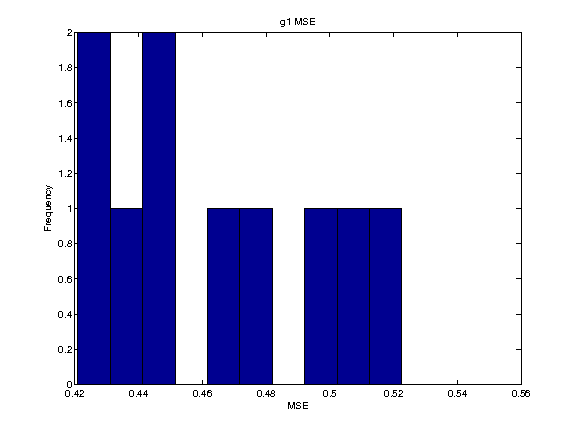
\includegraphics[width=\linewidth]{programming/g1-mse}
			\caption{Problem 5.a $g_1$ MSE}
			\end{subfigure}
			\begin{subfigure}{0.5\textwidth}
			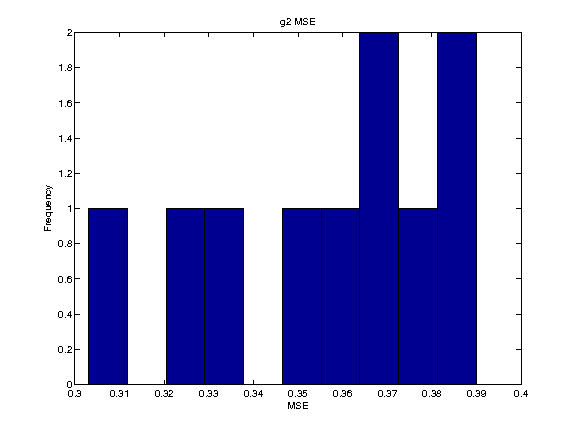
\includegraphics[width=\linewidth]{programming/g2-mse}
			\caption{Problem 5.a $g_2$ MSE}
			\end{subfigure}
		\end{figure} 
		
		\begin{figure}
			\begin{subfigure}{0.5\textwidth}
				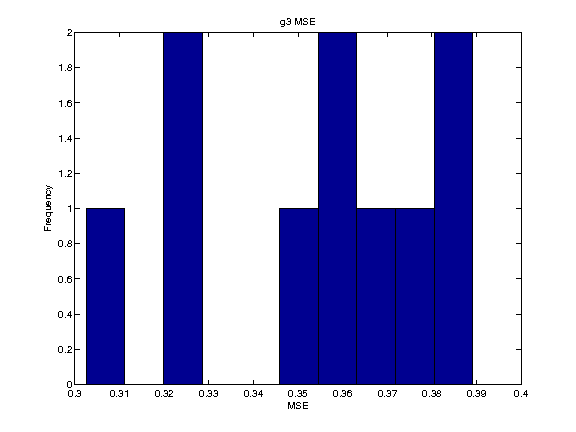
\includegraphics[width=\linewidth]{programming/g3-mse}
				\caption{Problem 5.a $g_3$ MSE}
			\end{subfigure}
			\begin{subfigure}{0.5\textwidth}
				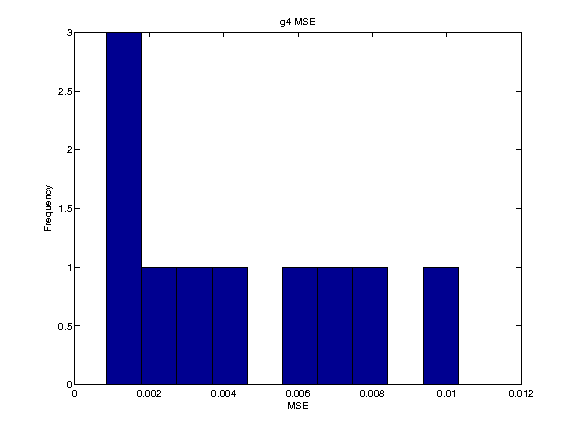
\includegraphics[width=\linewidth]{programming/g4-mse}
				\caption{Problem 5.a $g_4$ MSE}
			\end{subfigure}
		\end{figure} 
			
		\begin{figure}
			\begin{subfigure}{0.5\textwidth}
				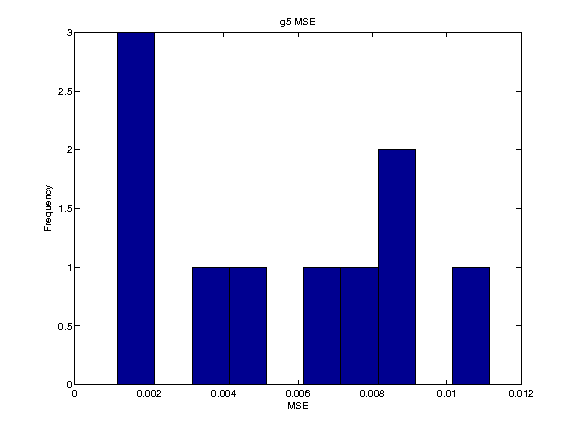
\includegraphics[width=\linewidth]{programming/g5-mse}
				\caption{Problem 5.a $g_5$ MSE}
			\end{subfigure}
			\begin{subfigure}{0.5\textwidth}
				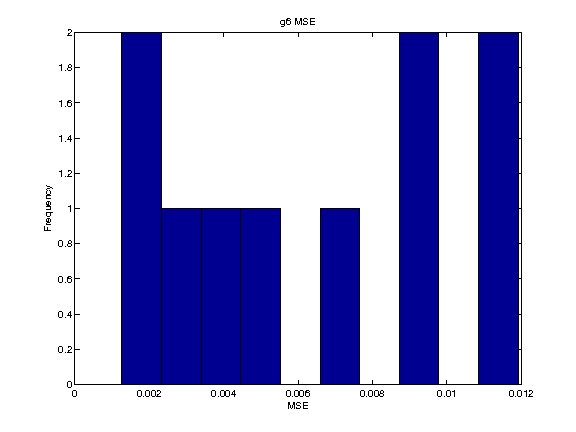
\includegraphics[width=\linewidth]{programming/g6-mse}
				\caption{Problem 5.a $g_6$ MSE}
			\end{subfigure}
		\end{figure} 
		
		
		
\end{homeworkSection}
\begin{homeworkSection}{\homeworkProblemName: ~(b)}
\problemAnswer{
		\begin{center}
			
			
			\begin{tabular}{|c|c|c|c|}
				\hline  $g$& $MSE$  & $Bias^2$  & $Variance$  \\ 
				\hline  $g_1$& 0.466517  & 0.118490 &  0.00\\ 
				\hline  $g_2$&  0.349509 & 0.003121  & 0.004464 \\ 
				\hline  $g_3$& 0.345009 & 0.003141 & 0.010835 \\ 
				\hline  $g_4$& 0.003469  & 0.000002  & 0.003411  \\ 
				\hline  $g_5$& 0.004510  & 0.000002 & 0.004441  \\ 
				\hline  $g_6$& 0.005375  & 0.000004  & 0.005292  \\ 
				\hline 
			\end{tabular} 
		\end{center}
	}
	\begin{figure}
		\begin{subfigure}{0.5\textwidth}
			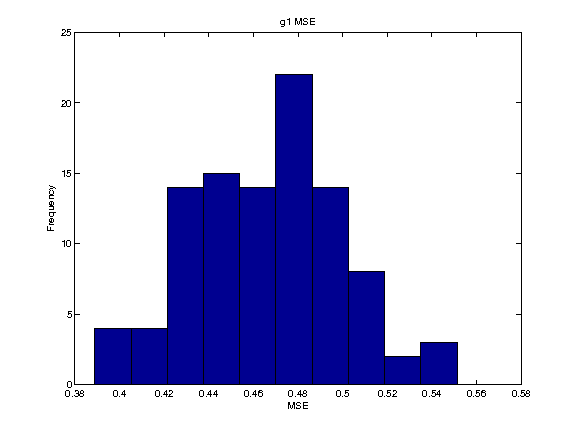
\includegraphics[width=\linewidth]{programming/g11-mse}
			\caption{Problem 5.b $g_1$ MSE}
		\end{subfigure}
		\begin{subfigure}{0.5\textwidth}
			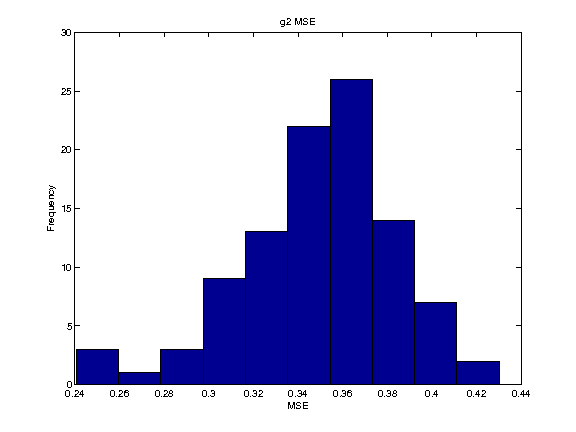
\includegraphics[width=\linewidth]{programming/g21-mse}
			\caption{Problem 5.b $g_2$ MSE}
		\end{subfigure}
	\end{figure} 
	
	\begin{figure}
		\begin{subfigure}{0.5\textwidth}
			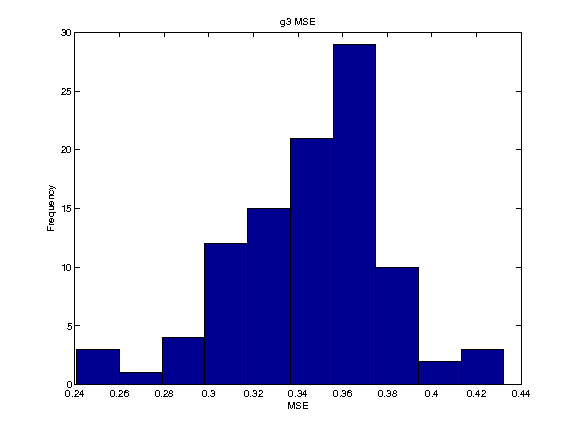
\includegraphics[width=\linewidth]{programming/g31-mse}
			\caption{Problem 5.b $g_3$ MSE}
		\end{subfigure}
		\begin{subfigure}{0.5\textwidth}
			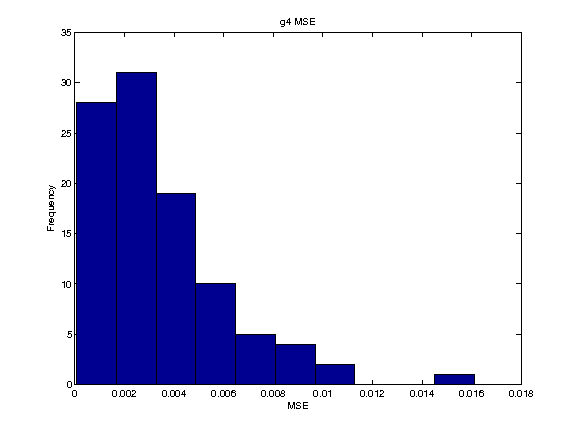
\includegraphics[width=\linewidth]{programming/g41-mse}
			\caption{Problem 5.b $g_4$ MSE}
		\end{subfigure}
	\end{figure} 
	
	\begin{figure}
		\begin{subfigure}{0.5\textwidth}
			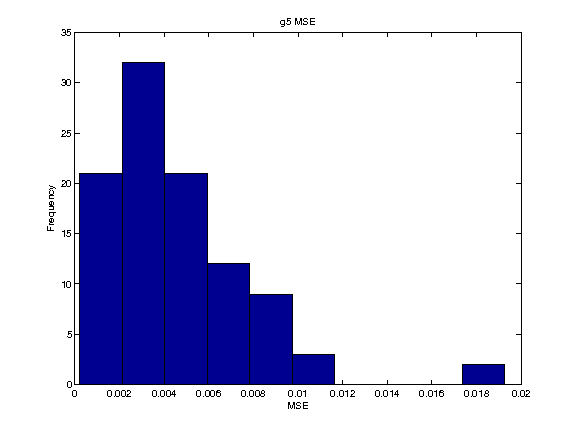
\includegraphics[width=\linewidth]{programming/g51-mse}
			\caption{Problem 5.b $g_5$ MSE}
		\end{subfigure}
		\begin{subfigure}{0.5\textwidth}
			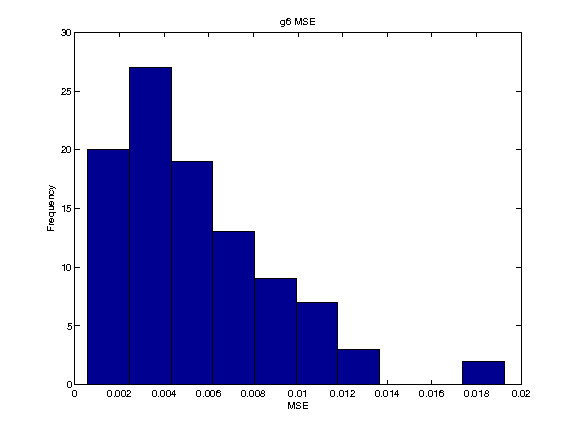
\includegraphics[width=\linewidth]{programming/g61-mse}
			\caption{Problem 5.b $g_6$ MSE}
		\end{subfigure}
	\end{figure} 
	
\end{homeworkSection}
\begin{homeworkSection}{\homeworkProblemName: ~(c)}
	\problemAnswer{
		As the model complexity increase the squared bias decreases  and the variance increases and the mean squared error decreases. However for some reason, the variance attributed with $g_3$ is a bit more than the normal trend. I could not think of a possible explanation for this.
		
		Another point to realise is that the variance is decreases for $g_4$ since it is a second order polynomial just like $f(x)=2x^2$.
		}

\end{homeworkSection}
\begin{homeworkSection}{\homeworkProblemName: ~(d)}
	\problemAnswer{
		\begin{center}
			
			
			\begin{tabular}{|c|c|c|c|}
				\hline  $lambda$ & $MSE$  & $Bias^2$  & $Variance$  \\ 
				\hline 0.01& 0.006682 & 0.000356 & 0.003399\\
				\hline 0.1& 0.014202 & 0.001268 & 0.003537\\
				\hline 1& 0.024060 & 0.002480 & 0.003716\\
				\hline 10& 0.035110 & 0.003843 & 0.003891\\
				\hline 
			\end{tabular} 
		\end{center}
		
		Thus, as the $\lambda$ increases the bias increases and the variance seems to increase too(unexpected, but anyway it is marginal). Since this is regularization problem, a higher $\lambda$ will try to further penalise the larger coefficients  and hence the coefficients tend to be close to zero, thus the bias increases. Ideally the variance should have decreased(again because the coefficients are now smaller!) but this does not seem to be reflected in my simulation.
		
		
		}
\end{homeworkSection}
\end{homeworkProblem}

\begin{homeworkProblem}[Problem 6]
	
\begin{homeworkSection}{\textbf{Linear Ridge Regression}}
		\problemAnswer{
			\centering
\begin{tabular}{|c|c|c|}
	\hline  Split& Optimal $\lambda$  & MSE  \\ 
	\hline  1& 0.01 &  0.016042 \\
	\hline  2& 0.0001 &   0.016664 \\
	\hline  3& 0 &   0.017038 \\
	\hline 
\end{tabular}
				\newline				\newline 
Mean test error: $0.016581$
			
			}
	\end{homeworkSection}
	
\begin{homeworkSection}{\textbf{Linear Kernel Ridge Regression}}
	\problemAnswer{
		\centering
		\begin{tabular}{|c|c|c|}
			\hline  Split& Optimal $\lambda$  & MSE  \\ 
			\hline  1& 0.01 & 0.016101   \\
			\hline  2& 0.0001 &  0.016829  \\
			\hline  3&  0.0& 0.017040    \\
			\hline 
		\end{tabular} 
		\newline\newline
		Mean test error: $0.016657$
		}
	\end{homeworkSection}
	
	\begin{homeworkSection}{\textbf{Polynomial Kernel Ridge Regression}}
			\problemAnswer{
			
			\centering
				\begin{tabular}{|c|c|c|c|c|}
					\hline  Split & Optimal $\lambda$  & Optimal $a$  & Optimal $b$ & MSE  \\ 
					\hline   1 &   0.01  &  0.5   &   2 &  $1.268206*10^{-02}$  \\ 
					\hline   2 &   1  &  0.0   &   3 &  $1.227860*10^{-02}$  \\ 
					\hline   3 &   10  &  1.0   &   3 &  $1.286726*10^{-02}$  \\ 
					\hline 
				\end{tabular} 
				\newline\newline
				Mean test Error: $0.012609$
			}
	\end{homeworkSection}
	
		\begin{homeworkSection}{\textbf{RBF Gaussian Kernel Ridge Regression}}
			\problemAnswer{
			\centering
				\begin{tabular}{|c|c|c|c|}
					\hline  Split & Optimal $\lambda$  & Optimal $\sigma^2$ & MSE  \\ 
					\hline  1 & 0.001 & 8 & 0.013382 \\ 
					\hline  2 & 0.01 & 8  & 0.012444 \\
					\hline  3 & 0.01 & 8  & 0.012080\\
					\hline 
				\end{tabular} 
				\newline\newline
				Mean test Error: $0.012635$
			}
		\end{homeworkSection}
		
	\begin{homeworkSection}{\textbf{Comparison}}


\problemAnswer{
	\textbf{Linear Ridge Regression mean test error} : $0.016581$
	
	\textbf{Linear Kernel Ridge Regression mean test error} : $0.016657$
		

	Kernel  ridge regression with linear kernel does not give the "same" results(they are very close though), and the thing to realise in this case is that linear kernel projects the data into $N \times N$ dimensions, while the ridge regression still has the 'kernel' in $D\times D$ dimensions. There is extra information being used here (in cases where $N>D$) In a a situation where $D>N$ the linear kernl might perform better.(I don't have a proof for this)
	
	\centering{
\begin{tabular}{|c|c|}
	\hline  Kernel &  Mean Test Error    \\ 
	\hline  Linear no Kernel & 0.016581 \\ 
	\hline  Linear Kernel &  0.016657 \\
	\hline  Polynomial Kernel &  0.012609 \\
	\hline  Gaussian Kernel & 0.012635  \\
	\hline 
\end{tabular} 
}
\newline

From the table we see, the Polynomial kernel with an average polynomial degree of $2.5$ performs the best, though Gaussian comes close. It looks like the poylnomial kernel in this case is better able to capture the non linearity in 2 or 3 dimensions, while the gaussian uses infinite dimensions.
	
	}
		\end{homeworkSection}
\end{homeworkProblem}

\end{document}
